\documentclass{article}
\usepackage{graphicx}
\usepackage{forest}
\usepackage{tikz}
\usepackage{float}
\usepackage{subcaption}
\usepackage{hyperref}
\usetikzlibrary{fit}
\graphicspath{ {./images/} }
\begin{document}
\title{An Implementation of Hypersuccinct Trees}
\author{Christopher Pack, Alexander Auras, Nathanael Stöhr, Charbono Lonyem Tegomo}
\date{\today}
\maketitle

%ADJUST FIGURE REFERENCES IN TEXT
%ADJUST FIGURE REFERENCES IN TEXT
%ADJUST FIGURE REFERENCES IN TEXT
%ADJUST FIGURE PLACEMENTS WHEN TEXT IS DONE
%ADJUST FIGURE PLACEMENTS WHEN TEXT IS DONE
%ADJUST FIGURE PLACEMENTS WHEN TEXT IS DONE

\begin{abstract}
This document describes a practical implementation of hypersuccinct tree encodings in C++. The theory is based on the procedures described in \cite{farzanMunro} and \cite{universalSuccinct}. A special focus lies on a space-efficient real-world-encoding and support of constant-time queries. We show that both of these constraints can be fulfilled in a practically usable implementation and provide a C++-library, Python-interface and GUI to showcase our results. We also summarize our findings regarding a short theoretical and practical analysis of the time- and space-requirements of an example service which reads, parses and writes XML-Files.

\end{abstract}

\tableofcontents

\section{Introduction}
Data storage is and has always been a challenge for multiple reasons, with the two probably most frequently occurring problems being access time and size. The challenges these problems pose only increase with more complex access mechanisms and datastructures.\\
One possible solution is the more efficient usage of the given space by the introduction of hypersuccinct data structures. Succinct data structures store data in some kind of compressed format, at or around the information-theoretical lower limit, while still allowing the execution of queries in an acceptable timeframe.\\
While much work has already been done on the theorecial site of things, the implementation of more complex succinct datastructures is not as well established. In this paper we present our practical implementation of hypersuccinct trees in C++ as an example of a complex hypersuccinct datastructure. The implementation should be space-efficient and still allow the execution of constant-time queries.\\
The theoretical basis for our implementation can be found in \cite{farzanMunro} and \cite{universalSuccinct}. While mainly a Proof-of-Concept, our library should also allow for easy extension and be usable as a solid basis-implementation of a hypersuccinct tree.

\section{The tree covering Algorithm}
To achieve the succinct encoding of the tree we follow the algorithm described by Farzan-Munro \cite{farzanMunro}. This algorithm has several steps. At first, the decompose-algorithm is used to divide the tree into several smaller subtrees of roughly equal size. These are called mini-trees. These mini-trees follow certain rules. Their nodes are disjoint, except they may have a common root node. Edges between mini-trees that do not share a common root node always end in the root node of the child tree and start from the root node of the parent tree, except for at most one edge in a mini-tree, that may start from any node in that tree and connect to the root of the child tree. We call this last special type of connection “dummy-interconnection”.\\
This allows to represent the interconnections of these subtrees with so called Fully Index-able Dictionaries (FIDs). Only the dummy-interconnections need their own handling. For these, we create a new dummy node on the interconnecting edge and store its pointer explicitly. Since there can at most be one such interconnection for each tree, the amount of created dummy nodes is bound by $O(log (n))$.\\
For the other types of interconnection, we distinguish between two types. Trees with type 1 interconnections share a common root node, while trees with type 2 interconnections are connected via an edge between their root nodes. With the FIDs and an additional vector we can represent both these interconnections. We create a FID for each root node. In the FID we store information about the child nodes of the root. This information allows us to identify which child nodes belong to a common tree. We use the additional vector, the Typevector (TV), to distinguish between interconnections of type 1 and type 2, by storing that information in 1 bit for each tree.\\
For each Mini-tree we store it's index in the FIDs and the data about its's Micro-trees together with some auxiliary information which will be described later. The size of this data of all Mini-trees is in $o(n)$ bits.

\subsection{Functions and Queries of the Hypersuccinct Tree}
To have a succinct data structure we have to be able to execute efficient query operations on our data. The auxiliary information stored for each Mini-tree is fundamental for that. In fact, the information we store allows us to execute many commonly needed query operations within $O(1)$ time. That means a lot of complex calculations are done upon creating the data and the results are then stored efficiently to be quickly available when asked for. \\

\begin{figure}[H]
\begin{tabular}{ |p{3.5cm}p{8cm}|} 
 \hline
 child($v$, $i$) & The $i$-th child of node $v$. \\
 childRank($v$) & The index of node $v$ as child of it's parent node. \\
 getParent($v$) & The parent node of node $v$. \\
 degree($v$) & The degree (number of children) of node $v$. \\
 subtreeSize($v$) & The size of the tree with node $v$ as root. \\
 depth($v$) &  The number of edges from the root to the node $v$. \\
 height($v$) & The number of edges from the node $v$ to the furthest leaf in it's subtree. \\
 leftmostLeaf($v$) & The leftmost leaf descendant of node $v$. \\
 rightmostLeaf($v$) & The rightmost leaf descendant of node $v$. \\
 leafSize($v$) & The number of leaf nodes in the subtree of node $v$. \\
 leafRank($v$) & The number of leaves before and including $v$. \\
 \hline
\end{tabular}
\caption{Queries of the Hypersuccinct Tree}
\label{2.1:table1}
\end{figure}

\section{Our Implementation}
This section is a short description of our implementation, which is made in C++.
%Do we need something here?

\subsection{Goals of the Implementation}
This library is mainly ment to provide some practical proof that the encoding offered by \cite{farzanMunro} and \cite{universalSuccinct} works in practice. Be mindful that our goal was to implement a succinctly encoded tree as described in \cite{farzanMunro}, with huffman encoding being the only part from \cite{universalSuccinct} impacting our project, therefore other changes described in \cite{universalSuccinct} are not part of this implementation.\\
This still results in a library that is ready for use in actual programs, so long as the limited implementation of functions actually suffices, and we discuss some of the shortcomings of this implementation in \textit{section 5}. This library is meant to be open and further refining and adding functionality should be possible and would be appreciated.\\
The library offers basic functionality around the hypersuccinct tree encoding such as generating a hypersuccinct tree from an .xml file, saving an encoded tree to a file and reading encoded files. The hypersuccinct tree offers a variety of queries, all implemented with a time complexity of $O(1)$.

\subsection{External Libraries}
We use four external libraries in our project.
The first one, called Irrxml \cite{irrXMLLink}, serves an implementation to read efficiently from an xml file. We use this library to generate a basic tree structure from xml files which is then used for our encoding.\\
We make use of a small library which provides an implementation of space efficient Fully Indexable Dictionaries \cite{universalSuccinct}, called succinct\_bv \cite{succinctBVLink}, which is implemented as described in \cite{succinctBV}.
This library is very lightweight and has been modified personally by us to suit our needs.\\
To increase the performance of our encoding process (see \textit{section 4.2}), we utilize a multithreading library called thread-pool \cite{threading}, to provide an efficient multithreading library.\\
Lastly, we utilise the googletest library \cite{googletestLink} for unit tests.

\section{Implementation in Depth}
We present our implementation in detail, and highlight issues we encountered during our implementation process and how we solved them.
\subsection{The Hypersucccinct Tree class}
The Hypersuccinct Tree class implements the entire hypersuccinct tree encoding. It consists of a struct representing minitrees and one representing the lookup table entries.
Both of these structs use plenty of bitvectors to store relevant data for queries.\\

Hypersuccinct Nodes:\\
Nodes within the Hypersuccinct Tree are identified as triplets, where the first value denotes the Minitree, the second the Microtree and the third the Node number within the Microtree.\\

\subsubsection{The FID and identifying trees}
FIDs represent the interconnections between trees at their roots, their type 1 and type 2 connections \cite{farzanMunro}, together with a Type Vector that shows which kind of connection the tree has.
Due to the way they are being generated, the FIDs do not share indices with their respective trees (i.e. it is possible for the Minitree with $id = 7$ to be in the FID with $id = 5$).
This necessitates an index conversion whenever the FID or the type vector is used. Doing this conversion at runtime would not be possible within $O(1)$, since it would be necessary to go through each FID and count the trees contained within it, for both type 0 and type 1 connections.
This is further complicated by taking into account the fact that each tree without dummies is actually accounted in two different FIDs. Firstly in the FID of its own root as a type 0 connection (Top FID), and secondly in the FID of its parent as type 1 (Low FID). Trees below dummies however have no low FID, as they are not directly below the root of their parent tree.
\begin{figure}[h]
	\begin{tabular}{ |p{3.5cm}||p{0.5cm}|p{0.5cm}|p{0.5cm}|p{0.5cm}|p{0.5cm}|p{0.5cm}|p{0.5cm}|p{0.5cm}|  }
		 \hline
		 \multicolumn{9}{|c|}{Vector indices for Trees} \\
		 \hline
		 Minitree Number & 0 & 1& 2 & 3 & 4 & 5 & 6 & 7\\
		 Minitree Top FID& 0 & 1 & 2 & 3 & 4 & 5 & 6 & 6\\
		 Minitree Low FID& - & 0 & 0 & 2 & 2 & 3 & - & -\\
		 \hline
	\end{tabular}
\caption{Indices for Minitrees}
\label{fid:table1}
\end{figure}
Therefore we implement a two way index conversion by directly pointing to the type 0 and type 1 FID index for each tree, and pointing to the first type 0 and type 1 tree for each FID. Since this is $O(4 \times |Minitrees|) + O(4 \times |Microtrees|)$, it is still within our required space complexity. Dummies on the other hand use direct pointers to their children.\\
\begin{figure}[h]
	\begin{tabular}{ |p{3.5cm}||p{1cm}|p{1cm}|p{1cm}|p{1cm}|p{1cm}|p{1cm}|p{1cm}|p{1cm}|  }
		 \hline
		 Bitvector & Bit 1 &Bit 2&Bit 3&Bit 4& Bit 5 &Bit 6&Bit 7&Bit 8\\
		 \hline
		 Minitree FID 0 & 1 & 1& 0 & 1 & 0 & 0 & 1 & 1\\
		 Minitree Typevector 0& 0 & 1 & - & 0 & - & - & 1 & 0\\
		 Minitree Numbers & 0 & 3 &  0 & 1 & 1 & 1 & 5 & 2\\
		 \hline
		 Minitree FID 1 & 1 & 0& 1 & 1 & 0 & 1 & 1 & 1\\
		 Minitree Typevector 1& 0 & - & 1 & 1 & - & 1 & 1 & 0\\
		 Minitree Numbers & 3 & 3 &  6 & 7 & 3 & 8 & 9 & 4\\
		 \hline
	\end{tabular}
\caption{FID, Typevector and corresponding trees}
\label{fid:table2}
\end{figure}
The second issue arises when trying to analyze the FID and Typevectors of the Hypersuccinct Tree. Identifying which tree is at which position within even a single FID is not trivial. As demonstrated in \textit{Figure 2}, the second low tree in the first FID is $5$, because the FID of tree $3$ contains tree $4$ already as a top tree, meaning correctly identifying Bit $7$ as tree number $5$ requires analysis of the FID of tree number $3$. Additionally, it is important to note that the FID with the ID of $1$ starts with the tree numbered $3$, which can only be known if all previous FIDs are also analyzed. Both of these computations exceed our time requirement of $O(1)$. Finding the first trees of any FID is clearly recursive starting from FID $0$, while correctly identfying low trees requires checking $|Low Trees|$ many additional FIDs. Therefore, the first top and low tree of any FID is pointed to directly.
This solves both of our issues, as the Rank of the Typevector indicates which FID belongs to which respective lower tree, allowing us to just take their first top tree as a result in $O(1)$. Knowing which tree an FID starts with is trivial with such pointers.


\subsubsection{The Hypersuccinct Tree Factory}
The Hypersuccinct Tree Factory is tasked with generating a hypersuccinct tree from our generic \textit{Unordered Tree} object, which is generated when reading an xml file. Additionally, the Factory also supports generating a tree directly from a full succinct Bitvector to support reading encoded files.\\
Encoding a generic tree is rather complicated due to the large amount of query related bitvectors that need to be filled with their respective data, a task that is not easily done on the generic tree structure. The complexity is therefore at least $O(|Nodes|^3)$, as we need to iterate through each minitree, within we iterate through each microtree, within we iterate through each node, as generated with the Farzan-Munro Algorithm by \cite{farzanMunro}. To increase the performance of this function, we make use of the multithreading library by \cite{threading}.\\
In contrast recreating a hypersuccinct tree from an encoded file is straightforward and easy. The data values from the file are just copied directly into their expected bitvector fields, which requires a complexity of $O(|Minitrees|) + O(|Lookup table entries|)$. Note that the file encoding is extremely space efficient and does not provide any ways to check if a given file is correctly encoded.\\
The Hypersuccinct Tree Factory generates all data necessary for query execution in $O(1)$, therefore fills all vector fields in Hypersuccinct Tree. The function is structured in loops and works as described in \cite{farzanMunro}. First, the Farzan Munro algorithm is executed on a base tree with the computed Minitree size of $\lceil log^2( |Nodes| ) \rceil$. Right after this, the Minitree interconnections are handled and Minidummies are generated. Then, the Farzan Munro algorithm is used on all generated Minitrees to generate their respective Microtrees of size $\lceil log( \frac{|Nodes|}{8} ) \rceil$, and their interconnections are handled. At last, for each of these Microtrees, a Lookup table entry is generated if an entry of such a tree sturcture does not already exist.\\
There are some special cases that lead to some additional complexity.

\begin{figure}[ht]
	\begin{subfigure}{3cm}
		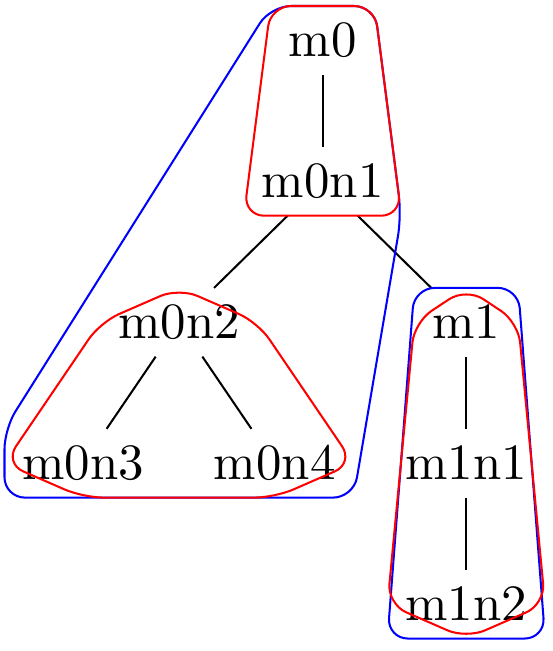
\includegraphics[scale=0.2]{F3C1Tree}
		\caption{Node order without Dummies}
		\label{factory:subim1}
	\end{subfigure}
	\begin{subfigure}{3cm}
		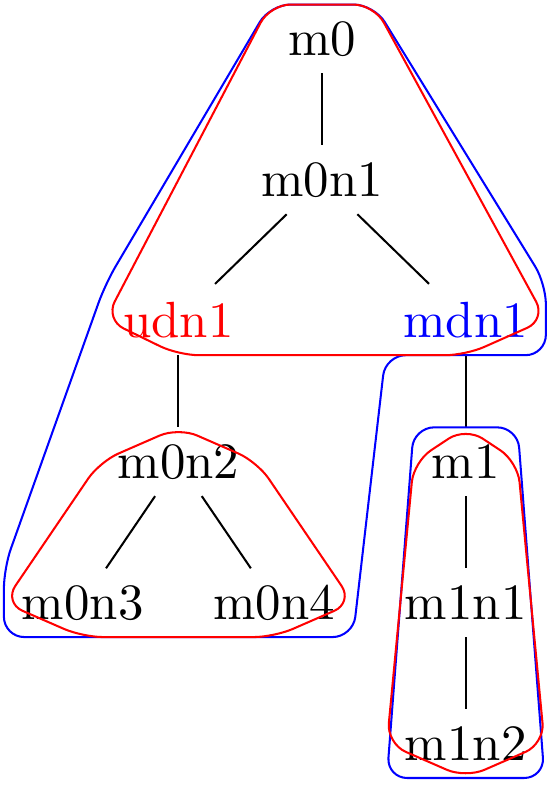
\includegraphics[scale=0.2]{F3C2Tree}
		\caption{Node order with Dummies}
		\label{factory:subim2}
	\end{subfigure}
	\begin{subfigure}{2.5cm}
		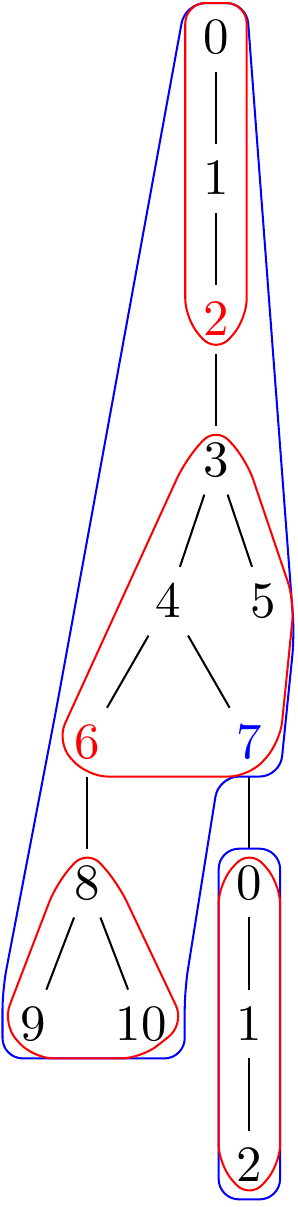
\includegraphics[scale=0.2]{F3C4Tree}
		\caption{Minitree specific node numbers}
		\label{factory:subim4}
	\end{subfigure}
	\begin{subfigure}{2.5cm}
		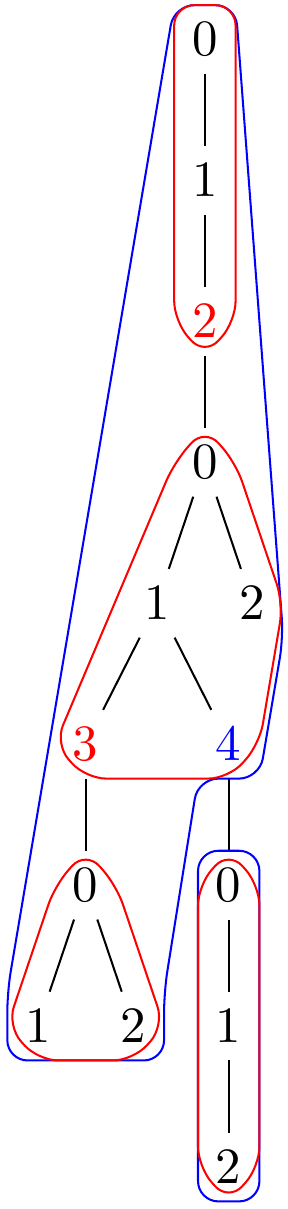
\includegraphics[scale=0.21]{F3C3Tree}
		\caption{Final Node numbers}
		\label{factory:subim3}
	\end{subfigure}

\caption{Special Cases regarding node order}
\label{factory:images4}
\end{figure}

The first issue originates from the handling of interconnections and the node numbering. Adding dummies in the Unordered Tree class does not retain the original structure of the nodes, especially when the Minidummy is located right after the Microdummy on the same level (\textit{Case a and b}). Therefore it becomes necessary to generate a consistent node numbering, which requires sorting the nodes within each tree. For this an \textit{enumerate} function is implemented that creates a consistent order for nodes within Mini and Microtrees.\\
Another issue is the identification of Minitree dummies within Microtrees. Minitree dummies are originally identified by their node number respective to the Minitree. However, due to the structure of Hypersuccinct nodes, it is necessary to translate the Minitree node numbers to Microtrees and Microtree node numbers. To solve this, we implemement a Microtree and node pointer for each Minitree dummy.

\subsection{Query structures and differences}
Not all queries represented in \cite{farzanMunro} are implemented. This is in part due to the simplicity of this implementation, but also because the original paper is rather shortworded when describing the implementation of each query, or simply points towards other papers related to this topic, which were not part of the scope of this implementation.
Due to this there are some minor or notable differences to the paper at hand, which will be elaborated on in this section.

\subsubsection{Simple Queries}
As simple Queries we identify those queries that only require a single bitvector per level of abstraction. This means that these queries need one bitvector for values of each Minitree, one for each Microtree within the Minitrees and one for each lookuptable entry.
As a result these queries all follow a similar structure, first handling single nodes, then generalizing the result to Microtrees and at last taking Minitrees into account to arrive at the correct result with an $O(1)$ time complexity.\\
These queries are:\\
\begin{itemize}
	\item[1)] \textit{getParent}
	\item[2)] \textit{degree}
	\item[3)] \textit{subtreeSize}
	\item[4)] \textit{depth}
	\item[5)] \textit{height}
	\item[6)] \textit{leftmostLeaf}
	\item[7)] \textit{rightmostLeaf}
	\item[8)] \textit{leafSize}
	\item[9)] \textit{levelSuccessor (Not implemented)}
	\item[10)] \textit{levelPredecessor (Not implemented)}
\end{itemize}
These queries are described as using one bitvector per abstraction in the paper. We therefore believe this implementation to be as described in the paper.\\
\textit{Depth} is specifically easy, since the depth of a given MicroTree or MiniTree root is just the size of their FIDs, making extra data bitvectors for depth unnecessary on a Minitree and Microtree level. All other queries use their respective bitvectors to determine a result.\\
\textit{getParent} is not directly mentioned as a query in \cite{farzanMunro}. Instead, when describing the \textit{childRank} query, it is mentioned that we first have to identify the parent of the given node. We decided to make this into a separate helper query, anticipating to need this query for some other queries as well. As we already had the helper query, we also made a normal query out of it.
On Dummies:\\
These queries require to handle the dummy in query-specific ways. \textit{Depth} is the simplest query, only adding values from Minitree depth, Microtree depth and Node depth. These do already ignore dummies in their data, so this query does not require any dummy handling. \textit{Height} and \textit{subtreeSize} make use of the \textit{isDummyAncestor} helper queries to subtract the dummy from their calculations. \textit{Degree}, \textit{leftmostLeaf} and \textit{rightmostLeaf} check whether or not the current node is the dummy, and then move along its pointer. \textit{GetParent} simply checks if the result is a dummy, and then returns the parent of that dummy. This is still within $O(1)$, as there are at most two dummies (one Microdummy and one Minidummy) on top of one another.\\
Despite not being implemented, we can still make some observations about 
\textit{levelSuccessor} and \textit{levelPredecessor}. Both cannot use the FID to compute their results, as identifying a specific node in the FID is not possible in $O(1)$. We therefore believe that a bitvector pointing to either the FIDs position or directly to the successor/predecessor is necessary, therefore making both of these Simple Queries. For dummies both would use the same handling as getParent, as the value returned by the dummy is the correct one, whereas the dummy's child would be effectively one level too low.

\subsubsection{Rank Queries}
Rank Queries are all queries that return some sort of rank from the tree. These queries are more compicated than Simple Queries since they require more than one bitvector per abstraction.
Rank queries specifically need two bitvectors for the Minitree and Microtree abstractions, due to special cases.
They also require use of the FID to identify these special cases.\\
The Rank Queries are:\\
\begin{itemize}
	\item[1)] \textit{childRank}
	\item[2)] \textit{leafRank}
	\item[3)] \textit{nodeRank (Not implemented)}
\end{itemize}
The first issue comes up regarding the identification of the given node within an FID. As the FID is structured it is not trivial to identify FID and the position of a node within the FID and would require $O(|TreesInFID|)$ time. To avoid this, our implementation uses the FID to identify the special cases and then take information from additional bitvectors.

\begin{figure}[ht]
	\begin{subfigure}{2cm}
		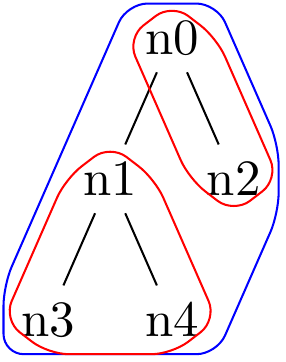
\includegraphics[scale=0.22]{F4C1Tree}
		\caption{Case 1}
		\label{rank:subim1}
	\end{subfigure}
	\begin{subfigure}{2cm}
		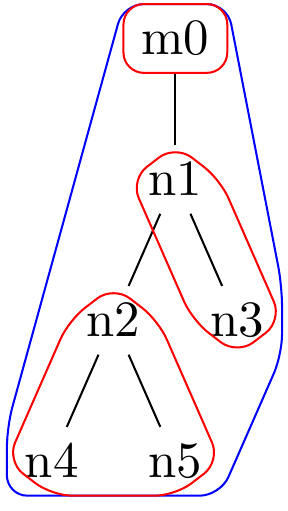
\includegraphics[scale=0.21]{F4C2Tree}
		\caption{Case 2}
		\label{rank:subim2}
	\end{subfigure}
	\begin{subfigure}{3cm}
		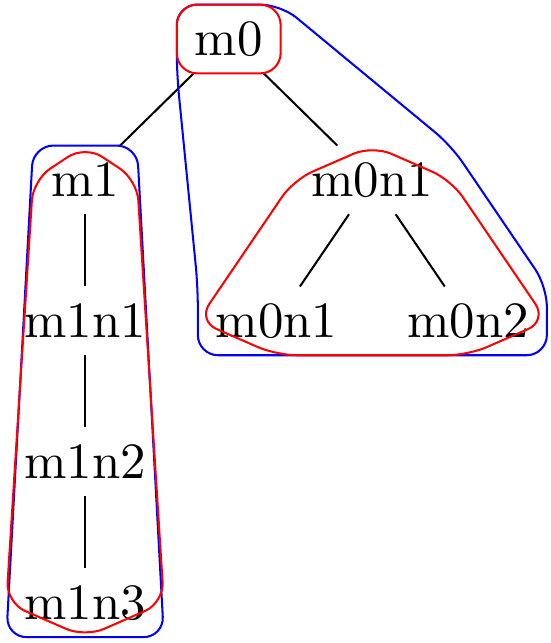
\includegraphics[scale=0.2]{F4C3Tree}
		\caption{Case 3}
		\label{rank:subim3}
	\end{subfigure}
	\begin{subfigure}{3cm}
		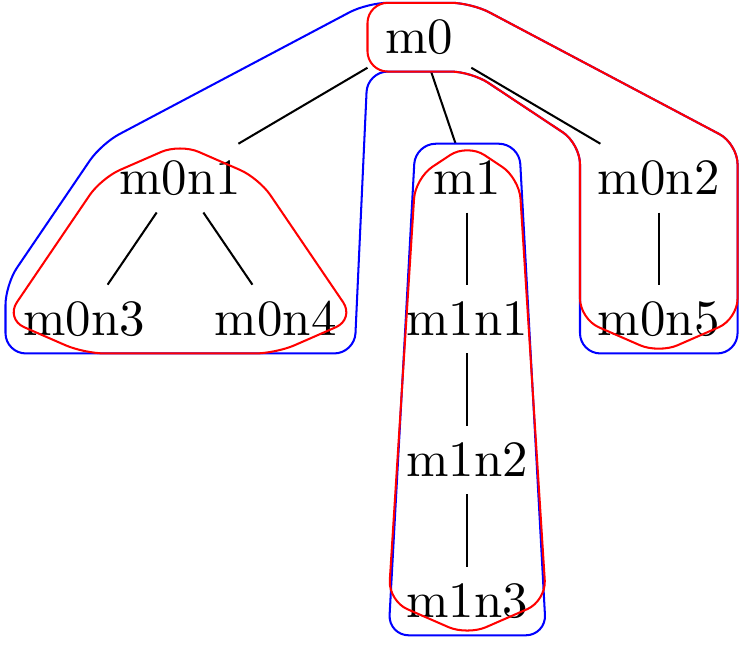
\includegraphics[scale=0.2]{F4C4Tree}
		\caption{Case 4}
		\label{rank:subim4}
	\end{subfigure}

\caption{4 Special Cases for Rank Queries}
\label{rank:images4}
\end{figure}

\begin{figure}[ht]
	\begin{tabular}{ |p{4cm}||p{1.5cm}|p{1.5cm}|p{1.5cm}|p{1.5cm}|  }
		 \hline
		 \multicolumn{5}{|c|}{Bitvectors} \\
		 \hline
		 Bitvector & Case 1 &Case 2&Case 3&Case 4\\
		 \hline
		 Minitree FID   & 1    & 1&   11 & 110\\
		 Minitree Typevector&   0  & 0   & 10 & 010\\
		 Microtree FID&11 &11&  irrelevant&irrelevant\\
		 Microtree Typevector&10& 10&  irrelevant&irrelevant\\
		 \hline
	\end{tabular}
\caption{FID and Typevector values for special cases}
\label{rank:table4}
\end{figure}

\textit{Case 1} and \textit{Case 2} describe a situation in which a higher indexed Microtree has a lower rank than the current Microtree. To resolve this, we introduce an extended rank bitvector which notes the rank of the first child of our current Microtree within the Minitree. This resolves this case on a data level, the second issue is to actually read the value of the extended bitvector in the right cases. This is where we differentiate between the two cases. If this problem appears at the Minitree root, we can identify this case by using the FID, resulting in \textit{Case 1}. If this problem appears further down in the Minitree we can compare values of Microtree and Node indices to identify \textit{Case 2}. \textit{Case 3} describes a similar issue regarding the Minitree. Again, a Minitree with a higher index has a lower rank than our current Minitree due to being a type 1 tree in the FID. This can also be identified with the FID. The three cases are mutually exclusive since they describe a similar issue.
\textit{Case 4} describes a tree of type 0 that is split by a tree of type 1 in between. This can be identified, since 0s in the FID must belong to the last type 0 tree, meaning after identifying the latest tree as being of type 1, one only needs to check if the index points to a 0 in the FID.\\
The structure of both queries is similar. First they calculate the result of only the node within the Microtree, using the values from the lookup table. Then, the result is generalized to a Microtree. Here, \textit{Case 2} is evaluated. At last, the result is generalized to the Minitree by analyzing key structures of the FID to identify \textit{Case 1}, or \textit{Case 3}. In \textit{childRank}, the special cases immediately return the value, as this query only needs to take into account the singular values of the parent FID. For \textit{leafRank}, a generalization to the entire tree is always necessary due to the result being sensitive to the entire tree topology.\\
Both implemented queries use \textit{getParentForQuery} as a helper query to identify the direct parent of the current node. These queries only check if the current node is a child of a dummy and if that is the case, the dummy is used instead, as the dummy is at the correct position to calculate the correct result.\\
These special cases are not mentioned in \cite{farzanMunro}. The description of all Rank Queries are rather short and fairly inconclusive.\\ 
It is for example correct that we use the FID to compute the childRank. However, we interpret the paper to say that computing the childRank is possible by just using the FID, without any additional data. 
Since this is not possible due to the identification of a node within the FID requiring $O(|Trees In FID|)$ time, our implementation uses the FID to identify the special cases. Both implemented Rank Queries also need to take their direct ancestor into account, which is not mentioned for LeafRank.
We believe our approach to be adequate, since both implemented queries fulfill the $O(1)$ time requirement without violating the space requirement. Additionally, both of our Rank Queries are very similar in their implementation offering easier understandability and openness, since adding \textit{nodeRank} would most likely just require the exact same steps as taken in our approach to Rank Queries.

\subsubsection{Child}
\textit{Child} is a more unique query. \textit{Child} is simpler than rank queries in principle, since the index provided by the query is directly related to an FID position, allowing an analysis of the node at that position in $O(1)$. It is important to note that identifying the correct child within the FID can point to a 0 value in the FID, and all issues for identifying nodes in the FID (\textit{Section 4.1.1}) apply here, making this query more complex.
This means that we need to identify Microtrees and nodes via the distance from the last $1$ within the respective FID of the Mini and Microtrees. To implement this, we first just identify the correct Minitree and reduce the remaining index by the position of that Minitree in the FID.
The process for identifying the Microtree is analogous to that, and at last we use the remaining index to select a specific node via the lookup table. If our starting node is already below the Minitree root, the part for identifying the right Minitree is skipped, same for Microtrees if we are below a Microtree root.
Dummy-nodes are skipped, both if the starting node is a dummy, in which case child of the direct pointer of the dummy is used instead, or if the result node is a dummy, in which case the direct pointer of the dummy is returned instead.\\
One thing we want to highlight is the identification of single nodes, below the Microtree. As \cite{farzanMunro} already describes, an Ancestor matrix is utilized for lookuptable entries (\textit{Section 4.2.4}). Therefore, we first implemented a child matrix alongside it, to identify children within Microtrees. We were however not able to identify a way to implement this task in $O(1)$ without making use of \textit{Rank} and \textit{Select} queries, requiring us to implement a FID for the matrix, increasing the space complexity.

\subsubsection{Helper Queries}
Instead of being identified by their algorithmic structure, these queries are identified by the fact that they are used by other queries to compute their results.\\
These Helper Queries are:
\begin{itemize}
	\item[1)] \textit{isDummyAncestorWithinMiniTree}
	\item[2)] \textit{isDummyAncestorWithinMicroTree}
	\item[3)] \textit{getParentForQuery}
\end{itemize}
Their implementation is similar to the implementation of Simple Queries.\\
\textit{GetParentForQuery} is a special version of \textit{getParent} that excludes handling for dummy nodes. This is necessary to identify special dummy cases in the queries that use this Helper Query (such as \textit{child}).
The \textit{isDummyAncestor} helper queries identify if a given node is an ancestor of a Minidummy or a Microdummy respectively. \textit{IsDummyAncestorWithinMiniTree} has a similar structure to the simple queries, first using specific bitvector data that contains if the Microtree root is an ancestor of the dummy, then if the specific node is the ancestor. \textit{IsDummyAncestorWithinMicroTree} is even simpler, only needing to determine the answer for specific nodes. Both queries are necessary to evaluate an entire tree structure in $O(1)$, since they prevent the necessity to analyze every node on the structure individually, which would be $> O(1)$. These queries utilize the lookuptable's ancestor matrix as described by \cite{farzanMunro}.

\subsubsection{Other Queries / Not implemented queries}
The following queries are not implemented and are not similar enough to already implemented queries to use those as a template. We briefly describe our issues with those queries.
\begin{itemize}
	\item[1)] \textit{nodeSelect (Not implemented)}
	\item[2)] \textit{levelAncestor (Not implemented)}
	\item[3)] \textit{lowestCommonAncestor (Not implemented)}
	\item[4)] \textit{distance (Not implemented)}
	\item[5)] \textit{levelLeftmostNode (Not implemented)}
	\item[6)] \textit{levelRightmostNode (Not implemented)}
\end{itemize}
Moving multiple levels is not trivial with our encoding. Since this is supposed to work in $O(1)$ time we are not sure how to implement a level based query. Moving up one level at a time is $> O(1)$, but adding one bitvector per level for each Microtree violates the space complexity requirement. This issue applies to queries \textit{2) to 6)}.\\
\textit{NodeSelect} has to call to a full mapping that orders all nodes with a single index, which is not how Hypersuccinct nodes are represented. Again, saving such a map for each Microtree and Minitree violates our space complexity requirement, but computing it violates the time complexity requirement.

\subsection{Other Classes}
There are a variety of other classes within the library that contribute to the functionality of our library.
\begin{itemize}
	\item[1)] \textit{Bitvector Utils}\\
			Bitvector Utils is a basic class that provides utility functions for Bitvectors. Its main function is to typecast Bitvectors to Integers and back, which is possible in $O(1)$ due to the limited size of Integers. (i.e. \textit{uint32\_t} has a maximum of $32$ bits.)
	\item[2)] \textit{HST Output}\\
			The HyperSuccinctTree Output class provides functions for writing and reading a Hypersuccinct Tree class. Therefore this class handles writing Hypersuccinct Trees to Files or reading Hypersuccinct Trees from Files. It also supports writing the entire tree into the console.
	\item[3)] \textit{Unordered Tree}\\
			Unordered Tree is our basic tree implementation, to which an xml tree is parsed. Unordered Trees are then used to create Hypersuccinct Trees.
	\item[4)] \textit{Precomputed Function and Cached Function}\\
			These two classes are used to improve the performance of the \textit{HypersuccinctTreeFactory}'s \textit{create} function by either completely precomputing values for queries within the Unordered Tree, or by caching already calculated values.
	\item[5)] \textit{XML Reader}\\
			This class reads the actual xml file and creates an Unordered Tree from it.
	\item[6)] \textit{Farzan Munro}\\
			The Farzan Munro class implements the algorithm as presented in \cite{farzanMunro}. It therefore implements \textit{decomopose} and \textit{greedilyPack}. It also orders the created Tree afterwards to guarantee a consistent order within the hypersuccinct tree.
\end{itemize}

\section{Runtime tests}
In order to test if our code fulfills the aforementioned boundaries of time we implemented several tests. Each of these tests first encodes a xml-file to a Hypersuccinct Tree, then runs several queries on up to 1000 nodes of the tree and records the time it takes to run for each run query. With these records we can show how fast the calls to each query where executed and calculate averages or boxplots. This, however, does not take into account the speed of the machine or other randomness effects related to the execution of the code on our computers.\\

\section{Complexity Benchmarks}
In this section we discuss some specific design decisions and shortcomings, and how they affect the performance of our hypersuccinct encoding.
\subsection{Huffman encoding}
\begin{figure}[h]
	\begin{tabular}{ |p{3cm}||p{2cm}|p{2cm}|p{4cm}|  }
		 \hline
		 Tree Name & Normal &Huffman &Huffman + Lookuptable\\
		 \hline
		 TreeNath.xml   & 52    & 23 &   24 \\
		 TreeNath2.xml&   484  & 256   & 266 \\
		 TreeNath3.xml&5196 &2695&  2706\\
		 TreeNath4.xml&53369& 31709&  31732\\
		 TreeNath5.xml&583289&345005&345029\\
		 XMark2.xml&2004196&831572&831627\\
		 DBLP.xml&3690039&593804&593842\\
		 \hline
	\end{tabular}
\caption{Space for normal encoding and huffman encoding}
\label{huff:table1}
\end{figure}
Our tree offers two types of encoding for Microtrees. The first option encodes trees according to \cite{farzanMunro}, and uses the Microtree's balanced parenthesis representation, while the other utilizes a huffman encoding for the Microtrees. For that, the Microtrees use their respective huffman codes in the representation, while their corresponding lookup table entries contain the balanced parenthesis representation for each code.\\
The huffman encoding has no impact on query performance, as finding a corresponding lookup table entry for a huffman code is possible in $O(1)$. Encoding trees with huffman has a significant impact on the space necessary for the Microtree encoding since the balanced parenthesis representation needs $2n$ many bits for a tree of size $n$, while huffman codes are more efficient (See Section 6.4).

\subsection{Factory Complexity}
The encoding process in \textit{create} is obviously not possible in $O(1)$, due to the Farzan-Munro algorithm itself being more complex, and the current implementation amounts to roughly $O(n^{3})$. Despite that we put significant effort into increasing the performance of the encoding process. The \textit{create} was evaluated in four separate options, whether or not to use huffman encoding, and whether or not to generate query data.\\
We in addition to that we also analyzed the runtime of \textit{writeToFile} and \textit{readFromFile}.
\begin{figure}[h]
	\begin{tabular}{ |p{3cm}||p{2,5cm}|p{2,5cm}|p{2,5cm}| }
		 \hline
		 Tree Name & Create & Write File &Read File\\
		 \hline
		 TreeNath.xml   & 00:00:00.056    & 00:00:00.003 &   00:00:00.026 \\
		 TreeNath2.xml&   00:00:00.081  & 00:00:00.003   & 00:00:00.023 \\
		 TreeNath3.xml&00:00:00.209 &00:00:00.033&  00:00:00.073\\
		 TreeNath4.xml&00:00:02.266& 00:00:00.308&  00:00:00.510\\
		 TreeNath5.xml&00:00:36.357&00:00:03.558&00:00:06.413\\
		 XMark2.xml&00:00:58.005&00:00:07.645&00:00:20.307\\
		 DBLP.xml&00:04:52.509&00:00:10.888&00:00:30.038\\
		 \hline
	\end{tabular}
\caption{Average runtimes for create, writing and reading files for specific trees}
\label{complexFac:table1}
\end{figure}
%Insert New image
\begin{figure}[h]
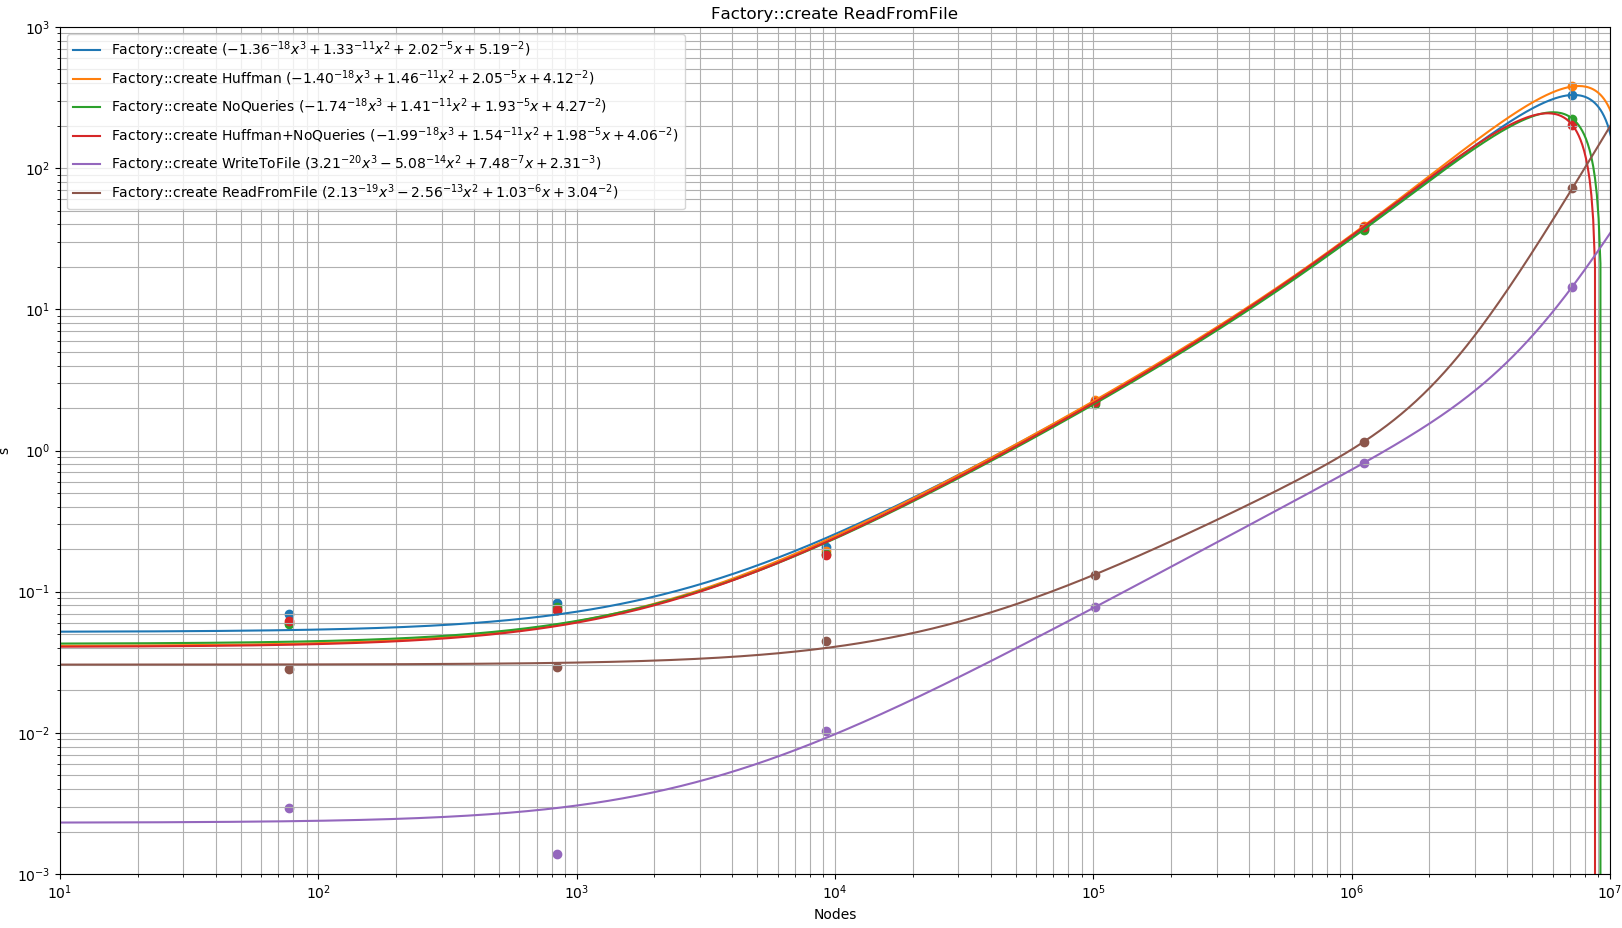
\includegraphics[scale=0.3]{file_compare_cut}
\caption{Runtime of \textit{create}}
\label{complexFac:image1}
\end{figure}

\subsection{Query complexity tests}
For query runtime tests we used \textit{DBLP}, which is a large, flat tree, and \textit{treeNath1-5}, which are trees of growing size and depth. The records we got from these tests show that queries on Hypersuccint Trees of vastly different size are still in the same magnitude of execution time. The longer execution times of larger trees compared to smaller trees can be accounted longer access times related to caching and hardware behaviour. The code itself maintains it's $O(1)$ execute time magnitude.\\
The queries provided by the hypersuccinct tree are implemented in $O(1)$, as specified in
\cite{farzanMunro}. As shown in \textit{Fig. 9} all queries except \textit{child} have an average runtime of well below $100 \mu s$. When it comes to \textit{child} when comparing between our different trees, the average runtime of \textit{child} increases with an increased amount of nodes. However, when analyzing our code, we were not able to find a section that would violate the $O(1)$ complexity requirement, not in our query implementation nor in the \textit{succinct\_bv} library. With some testing we determined that the increase in runtime stems from the basic function \textit{getMinitree}, which returns the Minitree for a given index, which is important for our evalutation, as hypersuccinct nodes save their Minitree as an integer (see Section 4.1).
Since this function simply calls the \textit{[]} operator of \textit{std::vector}, which per the C++ definition is $O(1)$. We argue that at some point a maximum runtime is reached and that this increase therefore does not violate our complexity requirement.
\begin{figure}[H]
\includegraphics[scale=0.3]{treeNath3_Queries}
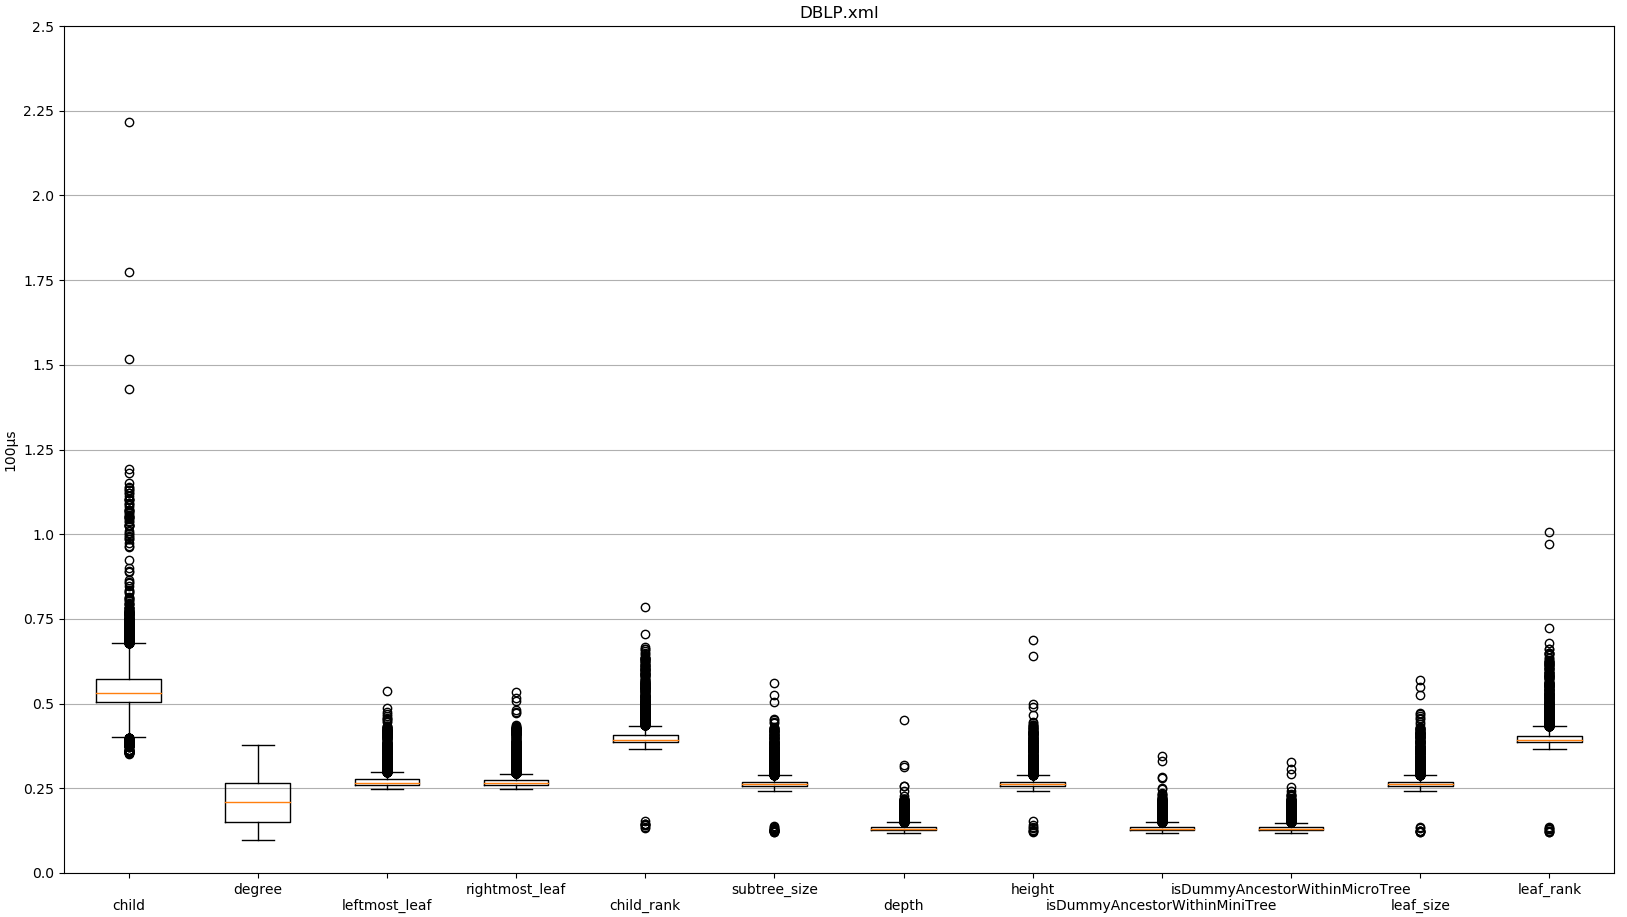
\includegraphics[scale=0.3]{DBLP_Queries}
\caption{Runtime of implemented queries}
\label{complexQue:image1}
\end{figure}

\subsection{Space complexity}
In this section we discuss the space complexity of our hypersuccinct tree implementation. For that matter let $n$ be the size of the entire tree, $m_{fm}$ be the calculated Minitree size of $\lceil lg^{2} n \rceil$, and $\mu_{fm}$ be the calculated Microtree size of $\lceil \frac{lg n}{8} \rceil$. Let this tree have $l$ many Minitrees, and let $m_{j}$ be the actual size of the j-th Minitree.

\subsubsection{Minitree Complexity}
Let $m$ be the size of a Minitree $M$ with $k$ many Microtrees $P$ and let $\mu_{i}$ be the size of its i-th Microtree $P_{i}$. Then we can describe the complexity of $M$ in the following way:\\

The amount of Microtrees $k$ is strictly dependent on $m$ and $\mu_{fm}$. As higher Microtree sizes reduce the number of Microtrees, the highest amount of Microtrees is reached when $\mu_{i} = 1$ $\forall i < k$, in which case $k = m$. It follows that $k \leq m$ \textit{(1)}.

The Microtrees are encoded in a vector, and there are two ways to encode them. If huffman encoding is enabled, the huffman code corresponding to the correct Lookuptable entry is used here, which has a complexity of $\leq O(m)$, as shown in \cite{universalSuccinct} %This is not shown directly. Terefore this might not suffice as an argument.
If huffman encoding is disabled, the Microtrees are encoded in balanced parenthesis form, which takes $2\mu_{i}$ many bits for Microtree $i$.\\
This leads to a total of $\displaystyle\sum_{i=0}^{k-1} 2 \times \mu_{i}$. \textit{(2)}\\
Given that due to their construction the Microtrees can share roots, the worst possible outcome would be that all trees share the same root, in which case \textit{(2)} $= 2(m + k)$. The maximum amount of Microtrees possible (that can still share roots) is reached when the size of all Microtrees is $= 2$, in which case \textit{(2)} $= 4m = 4k$. Therefore, \textit{(2)} $\leq 4m \in O(m)$.

Microtree dummys and the Microtree-to-FID index conversion vector, as well as any query vector related to Microtrees all have $k$ many entries, and both of them encode integers which is possible in $O(1)$. From \textit{(1)} if follows that all these vectors have a complexity of $\leq O(m)$. Any query data related to the Minitree itself is a single encoded integer, and therefore $O(1)$.

The Microtree FIDs, Typevectors, and FID-to-Microtree index conversion vector have one entry for each FID, and there is only one FID for each unique Microtree root. Therefore let there be $f$ many Microtree FIDs. Then, $f \leq k$, where $f = k$ if $k = m$, because then every tree consists of a single node and that node is a unique root.
While the index conversion vector saves integers in $O(1)$ and therefore has a complexity of $O(m)$, the FIDs and Typevectors however save data depending on the amount of children of a Microtree root.\\
This therefore amounts to $\displaystyle\sum_{i=0}^{k-1} \textit{degree(root($P_{i}$))}$ \textit{(3)}.\\
Since the the Minitree is of size $m$, it follows that $\sum_{i=0}^{k-1} \textit{degree(root($P_{i}$))} = m-1$, since the degree of all leaves is $0$ and, starting from the Minitree root, there are only $m-1$ many children in total.
Therefore it follows that \textit{(3)} $\leq \sum_{i=0}^{k-1} m = k \times m$, and due to \textit{(1)} it follows that \textit{(3)} $\leq m^{2}$, which has a complexity of $O(m^{2})$.

The Microtree FIDs and Typevectors also implement \textit{Rank} and \textit{Select} using the procedure in \cite{succinctBV} and \cite{succinctBVLink}. Let $\xi_{u}$ be the size of the u-th FID.
The complexity for this FID is described as $\xi_{u} + O(\frac{\xi_{u} log log \xi_{u}}{log \xi_{u}})$.\\
Since there are at most $k$ many FIDs, this amounts to 
$$\displaystyle\sum_{i=0}^{k-1} \textit{degree(root($P_{i}$))} + O(\frac{(\textit{degree(root($P_{i}$)))} log log (\textit{degree(root($P_{i}$)))}}{log (\textit{degree(root($P_{i}$)))}})$$\\
$$\leq O(m^{2}) + O(\frac{(\textit{degree(root($P_{i}$)))} log log (\textit{degree(root($P_{i}$)))}}{log (\textit{degree(root($P_{i}$)))}})$$\\
$$\leq O(m^{2}) + O(\frac{m log log m}{log m})$$

\subsubsection{Lookuptable complexity}
Let the lookuptable entry $LP_{h}$ have size $\mu_{h}$. Then its complexity can be described as follows:\\

The first two bitvectors encode the structure of the tree.
If huffman encoding is enabled, then the index vector saves the huffman code of this entry $C_{h}$, which has a complexity of $\leq O(m)$, as shown in \cite{universalSuccinct} %This is not shown directly. Terefore this might not suffice as an argument.
In both cases, the balanced parenthesis form of the entry is saved, which has a complexity of $O(\mu_{h})$.

The lookuptable entry saves query data for each node within its structure, which has a complexity of $O(\mu_{h})$.
The lookuptable then saves two specific matrices for query data, both of which have a complexity of $O((\mu_{h})^{2})$.
One of these two also requires \textit{Rank} and \textit{Select} queries, their implementation has a complexity of 
$$(\mu_{h})^{2} + O(\frac{(\mu_{h})^{2} log log (\mu_{h})^{2}}{log (\mu_{h}})^{2})$$\\
$$\in O((\mu_{h})^{2}) + O(\frac{(\mu_{h})^{2} log log (\mu_{h})^{2}}{log (\mu_{h}})^{2})$$

\subsubsection{Total space complexity}
Coming together for the entire tree, let $n$ be the size of the entire tree, $m_{fm}$ be the calculated Minitree size, and $\mu_{fm}$ be the calculated Microtree size. Let this tree have $l$ many Minitrees, and let $m_{j}$ be the actual size of the j-th Minitree, then for a hypersuccinct tree $N$ of size $n$, the complexity can be described in the following way:\\

The tree saves a flag for huffman encoding, its own size $n$, and the Minitree size $m_{fm}$ and the Microtree size $\mu_{fm}$.\\

Just as within the Minitrees, the amount of Minitrees $l$ is per construction directly correlated to the tree size $n$. If $\forall j < l:$ $m_{j} = 1$, and in that case $l = n$, and therefore $l \leq n$ \textit{(1)}\\

The tree then saves vectors for the Minitree FIDs, Typevectors, Dummys and index conversions between the FIDs and Minitrees, and their complexity is analoguos to their Microtree counterparts. Therefore the Minitree FIDs and Typevectors have a complexity of $O(n^2)$, the dummys and index conversions all have a complexity of $O(n)$.
Support for \textit{Rank} and \textit{Select} for FIDs and Typevectors have a complexity of $O(n^{2}) + O(\frac{n log log n}{log n})$.\\

When it comes to the Minitrees, there are obviously $l$ many Minitrees, and each Minitree $j$ has a complexity of $O(m_{j}^{2}) + O(\frac{m_{j} log log m_{j}}{log m_{j}})$.
Therefore the entire structure has a size of $\displaystyle \sum_{b=0}^{l} (O(m_{b}^{2}) + O(\frac{m_{b} log log m_{b}}{log m_{b}}))$.\\
Analogously to Microtrees, all Minitrees can share roots, or have a dummy (in which case the tree below has a unique root), therefore  $\sum_{b=0}^{l-1} m_{b} \leq 2n$,
therefore 
$$\displaystyle \sum_{b=0}^{l} (O(m_{b}^{2}) + O(\frac{m_{b} log log m_{b}}{log m_{b}}))$$\\ 
$$\leq \displaystyle O(2n^{2}) + O(\frac{2n log log 2n}{log 2n})$$\\ 
$$= O(n^{2}) + O(\frac{n log log n}{log n})$$

When it comes to the Lookuptable, the amount of entries is less or equal to the amount of unlabeled ordered trees of size $2 \times \mu_{fm}$ or less, which is the sum of the Catalan Numbers $\sum_{v=1}^{2\mu_{fm}} Ca(v) = \sum_{v=1}^{2\mu_{fm}} \sum_{c=0}^{v} a(c)a(v-1-c)$, as shown in \cite{catalanN}. A lookuptable entry $h$ then has a size of $\mu_{h}$, and a complexity of $O((\mu_{h})^{2}) + O(\frac{(\mu_{h})^{2} log log (\mu_{h})^{2}}{log (\mu_{h})^{2}})$. Since the lookuptable only saves unique entries with a unique structure, the worst possible case in terms of space can only be when each tree structure is only used exactly once. In that case each entry $h$ directly maps to a Microtree $\mu$, and the sum of all Microtrees sizes in a Minitree is $\leq 2m$. Then, since the sum of all Minitree sizes is $\leq 2n$, the sum of all Microtrees in the entire tree is $\leq 4n$, and this is also true for the sum of all lookuptable entry sizes.
Therefore the total complexity of all entries is
$$\sum_{v=1}^{2\mu_{fm}} (Ca(v) \times (O(v^{2}) + O(\frac{v^{2} log log v^{2}}{log v^{2}})))$$
$$\leq O((4n)^{2}) + O(\frac{(4n)^{2} log log (4n)^{2}}{log (4n)^{2}})$$
$$ = O(n^{2}) + O(\frac{n^{2} log log n^{2}}{log n^{2}})$$

%In the worst case, these should all be =, and therefore this should be the FINAL CORRECT Complexity
%This complexity seems too high...


\subsubsection{Space Complexity concessions}
While the encoding is efficient in size when saving a tree to a file, within the program, the amount of space required to run trees is a lot larger. This technically does not break the space complexity, simply adding a large constant factor to it, but this is still notable. We identify the following reasons for this discrepancy:\\
\begin{itemize}
	\item[1)] The implementation of \textit{Bitvector} in $C++$ saves its data as \textit{uint32\_t}, which is always 32 bits long. This is a massive waste of space, since most values are much smaller than 32 bits.
	\item[2)] The \textit{succinct\_bv} library does not meet the perfect space complexity from \cite{succinctBV} of $log(\begin{array}{c} n \\ r \end{array}) + O(\frac{n log log n}{log n})$, and instead has a complexity of $n + O(\frac{n log log n}{log n})$ for a bitvector of size $n$.
\end{itemize}
For \textit{1)}, we believe it to be possible to save the entire hypersuccinct tree in a single bitvector. It should be possible to use pointers to access different parts of this bitvector in $O(1)$ using a variable cell array, as described in \cite{universalSuccinct}.\\
For \textit{2)}, it is obviously necessary to either use a library that offers the improved complexity, or to improve the current library.

\section{Conclusion}
In this work we demonstrated that an implementation of a hypersuccinct tree is not only possible, but also usable in real-world scenarios. Both a theoretical analysis and a practical evaluation of a test service have shown that the space-efficiency of our implementation is sufficiently high, and follows the instructions presented in \cite{farzanMunro}. We were also able to implement queries in a constant time.\\
Also noteworthy is the effect of the application of the Huffman encoding for microtree-representation, which further improves the space-complexity by a significant amount.\\
Further work could be done by implementing some missing complex and underspecified queries. Additional optimization potential regarding the memory-footprint of our library also exists (e.g. merging bitvectors together).\\
Nonetheless, our example applications show that our implementation is more than sufficient to process common Use-Cases, such as loading a tree from an existing file, parsing another tree format to a hypersuccinct tree, visualizing the tree and queries and saving the results back to a file.

\section{Data}
All trees can be found in the resources folder of our project on Github, on \href{https://github.com/ChristopherPack/Projektgruppe\_Hypersuccint\_Trees}{https://github.com/ChristopherPack/Projektgruppe\_Hypersuccint\_Trees}, or on \href{http://xmlcompbench.sourceforge.net/Dataset.html}{http://xmlcompbench.sourceforge.net/Dataset.html}.
\subsection{Used xml tree files}
\begin{figure}[H]
	\begin{tabular}{ |p{3cm}||p{2,5cm}||p{2,5cm}| }
		 \hline
		 Tree Name & Size & Depth\\
		 \hline
		 TreeNath.xml   &77 & 8\\
		 TreeNath2.xml&  837 & 31\\
		 TreeNath3.xml&9197 & 119\\
		 TreeNath4.xml&101157 & 228\\
		 TreeNath5.xml&1112717 & 351\\
		 XMark2.xml&3603803 & 12\\
		 DBLP.xml&7146530 & 6\\
		 \hline
	\end{tabular}
\caption{sizes of our xml trees}
\label{data:table1}
\end{figure}

\bibliographystyle{IEEEtran}
\bibliography{references}

\end{document}
